\chapter{Methodik}
\label{ch:methodik}

FMOE fällt in die dritte Kategorie und unterscheidet sich von anderen Verfahren derselben Kategorie hauptsächlich durch die Verwendung von FM-Index und damit verbundenen Optimierungen.

Im Folgenden werden daher zuerst die Datenstrukturen behandelt.

\section{Datenstrukturen}
\label{sec:datenstrukturen}

Der FM-index ist eine Datenstruktur für Zeichenfolgen, die auf der Burrows Wheeler Transformation (BWT) basiert.

Die BWT ist ein Algorithmus, der aus einer beliebigen Zeichenfolge eine Permutation dieser Folge und einen Index erzeugt, mit dem Effekt, dass die erhaltene Permutation in der Regel leichter zu komprimieren ist.
Eine Rücktransformation ermöglicht dann die Wiederherstellung der ursprünglichen Zeichenfolge.
%TODO:Quelle Burrows Wheeler Transform

Der FM-Index wird ähnlich zur BWT konstruiert, speichert aber zusätzliche Daten, um schnelle Patternsuche bei immer noch sehr geringer Speicherkomplexität zu ermöglichen.
Die Funktionsweise und die Gründe für die Resourcensparsamkeit lassen sich am besten im Vergleich zum Suffix-Array erläutern.

\newcolumntype{a}{>{\color{gray}}c}
\newcolumntype{b}{>{\columncolor{lightgray}}c}
\begin{figure}[h]
	\begin{center}
		\begin{tabular}{ c || c c c c c c c c c c | }
			\hline
			0 & a & t & g & a & t & t & a & t & c & \$ \\
			\hline
			1 & t & g & a & t & t & a & t & c & \$ &   \\
			\hline
			2 & g & a & t & t & a & t & c & \$ &   &   \\
			\hline
			3 & a & t & t & a & t & c & \$ &   &   &   \\
			\hline
			4 & t & t & a & t & c & \$ &   &   &   &   \\
			\hline
			5 & t & a & t & c & \$ &   &   &   &   &   \\
			\hline
			6 & a & t & c & \$ &   &   &   &   &   &   \\
			\hline
			7 & t & c & \$ &   &   &   &   &   &   &   \\
			\hline
			8 & c & \$ &   &   &   &   &   &   &   &   \\
			\hline
			9 & \$ &   &   &   &   &   &   &   &   &   \\
			\hline
		\end{tabular}
		\caption{Suffixe}%
		\label{tbl:suffixes}
	\end{center}
	\begin{center}
		\begin{tabular}{ c || c c c c c c c c c c | }
			\hline
			0 & a & t & g & a & t & t & a & t & c & \$ \\
			\hline
			1 & t & g & a & t & t & a & t & c & \$ & a \\
			\hline
			2 & g & a & t & t & a & t & c & \$ & a & t \\
			\hline
			3 & a & t & t & a & t & c & \$ & a & t & g \\
			\hline
			4 & t & t & a & t & c & \$ & a & t & g & a \\
			\hline
			5 & t & a & t & c & \$ & a & t & g & a & t \\
			\hline
			6 & a & t & c & \$ & a & t & g & a & t & t \\
			\hline
			7 & t & c & \$ & a & t & g & a & t & t & a \\
			\hline
			8 & c & \$ & a & t & g & a & t & t & a & t \\
			\hline
			9 & \$ & a & t & g & a & t & t & a & t & c \\
			\hline
		\end{tabular}
		\caption{Rotationen}%
		\label{tbl:rotations}
	\end{center}
	\caption{Vorstufen von Suffix-Array und FM-Index für die Zeichenfolge \glqq atgattatc\$\grqq}
	\label{fig:construction}
\end{figure}

\begin{figure}[h]
	\begin{center}
		\begin{tabular}{ c || c c c c c c c c c c | }
			\hline
			9 & \$ &   &   &   &   &   &   &   &   &   \\
			\hline
			6 & a & t & c & \$ &   &   &   &   &   &   \\
			\hline
			0 & a & t & g & a & t & t & a & t & c & \$ \\
			\hline
			3 & a & t & t & a & t & c & \$ &   &   &   \\
			\hline
			8 & c & \$ &   &   &   &   &   &   &   &   \\
			\hline
			2 & g & a & t & t & a & t & c & \$ &   &   \\
			\hline
			5 & t & a & t & c & \$ &   &   &   &   &   \\
			\hline
			7 & t & c & \$ &   &   &   &   &   &   &   \\
			\hline
			1 & t & g & a & t & t & a & t & c & \$ &   \\
			\hline
			4 & t & t & a & t & c & \$ &   &   &   &   \\
			\hline
		\end{tabular}
		\caption{Suffix-Array}
		\label{tbl:suffix-array}
	\end{center}
	\begin{center}
		\begin{tabular}{ c || b a a a a a a a a b | }
			  & \cellcolor{white} F &   &   &   &   &   &   &   &   & \cellcolor{white}L \\
			\hline
			\hline
			9 & \$ & a & t & g & a & t & t & a & t & c$_1$ \\
			\hline
			6 & a$_1$ & t & c & \$ & a & t & g & a & t & t$_1$ \\
			\hline
			0 & a$_2$ & t & g & a & t & t & a & t & c & \$ \\
			\hline
			3 & a$_3$ & t & t & a & t & c & \$ & a & t & g$_1$ \\
			\hline
			8 & c$_1$ & \$ & a & t & g & a & t & t & a & t$_2$ \\
			\hline
			2 & g$_1$ & a & t & t & a & t & c & \$ & a & t$_3$ \\
			\hline
			5 & t$_1$ & a & t & c & \$ & a & t & g & a & t$_4$ \\
			\hline
			7 & t$_2$ & c & \$ & a & t & g & a & t & t & a$_1$ \\
			\hline
			1 & t$_3$ & g & a & t & t & a & t & c & \$ & a$_2$ \\
			\hline
			4 & t$_4$ & t & a & t & c & \$ & a & t & g & a$_3$ \\
			\hline
		\end{tabular}
		\caption{FM-Index}
		\label{tbl:fm-index}
	\end{center}
	\caption{Resultierender Suffix-Array und FM-Index für die Zeichenfolge \glqq atgattatc\$\grqq}
	\label{fig:finished}
\end{figure}

Wie in den Tabellen \ref{tbl:suffixes} und \ref{tbl:rotations} zu sehen ist, beginnt man bei beiden Datenstrukturen damit, alle Suffixe der Zeichenfolge zu erzeugen.
Im Fall des FM-Index wird jede Zeile mit dem Anfang der Zeichenfolge aufgefüllt, sodass sich die Rotationen der Zeichenfolge ergeben.
Zusätzlich werden die Suffixpositionen in der Zeichenfolge in einer extra Spalte festgehalten.

Das Ergebnis dieser Operation wird dann lexikographisch sortiert. In Tabelle \ref{tbl:suffix-array} ist der fertige Suffix Array zu sehen.
Während bei dem Suffix-Array das gesamte Array gespeichert werden muss, kann beim FM-Index auf einen großen Teil der Daten verzichtet werden.

\begin{itemize}
	\item Aus den Rotationen müssen nur die Spalten F und L gespeichert werden.
	\item Die Spalte F ist aufsteigend sortiert und kann daher bei einem kleinen Alphabet wie $\{A, C, G, T, \$\}$ sehr stark komprimiert werden.
	\item Für den Suchalgorithmus müssen die Ränge der Zeichen in der letzten Zeile (in Tabelle \ref{tbl:fm-index} als tiefgestellte Indizes sichtbar) bekannt sein.
		Diese kann man bei jeder Suche neu berechnen oder speichern.
		In den meisten Fällen wird ein hybrider Ansatz verwendet, bei dem ein Bruchteil der Ränge vorberechnet und gespeichert wird, um die Berechnung der Übrigen zu beschleunigen.
	\item Die Positionen in der usprünglichen Zeichenfolge (in den Tabellen \ref{fig:finished} als getrennte Spalte sichtbar) können genau wie die Ränge teilweise vorberechnet werden, um einen guten Kompromiss zwischen Speicherverbrauch und Rechenaufwand zu erhalten.
\end{itemize}

Diese Optimierungen sorgen dafür, dass ein Suffix-Array in der Regel ein vielfaches an Speicher benötigt als ein FM-Index.

\subsection{Patternsuche}
\label{subsec:patternsearch}

Die Patternsuche im Suffix-Array ist trivial, da es für jedes Vorkommen des Patterns einen Suffix geben muss, der mit dem Pattern beginnt.
Weil alle Suffixe lexikographisch sortiert sind, liegen alle Suffixe, die mit dem Pattern beginnen hintereinander im Array.
Es genügt also den Ersten und den Letzten der Suffixe durch wiederholte binäre Suche zu finden und mithilfe der ersten Spalte die Position aller dazwischen liegenden herauszufinden.
\\
Beispiel: Suche nach \glqq att\grqq (siehe auch Tabelle \ref{tbl:suffix-array-search})
\begin{enumerate}
	\item Durch binäre Suche das Intervall der Suffixe finden, dass mit \glqq a\grqq beginnt (blau).
		Wenn die erste Spalte des Arrays durch RLE\footnote{RLE steht für Run Length Encoding (auf Deutsch Lauflängenkodierung) und ist eine Kompression, die bei Daten mit vielen Symbolwiederholungen eingesetzt wird. Beispiel: \glqq aaaaabbb\grqq wird komprimiert zu \glqq a5b3\grqq}
		komprimiert wurde, kann dieser Schritt ohne binäre Suche in konstanter Zeit stattfinden.
	\item Mit binärer Suche das Teilintervall finden, dessen zweites Zeichen \glqq t\grqq ist (orange).
	\item Schritt 2 für das nächste Zeichen wiederholen (rot).
	\item Den gefundenen Suffix anhand der extra Spalte seiner Position in der Zeichenfolge zuordnen (Index 3)
\end{enumerate}

\begin{figure}[h]
	\begin{center}
		\begin{tabular}{ c || c c c c c c c c c c | }
			\hline
			9 & \$ &   &   &   &   &   &   &   &   &   \\
			\hline
			6 & \cellcolor{SkyBlue} a & \cellcolor{BurntOrange} t & c & \$ &   &   &   &   &   &   \\
			\hline
			0 & \cellcolor{SkyBlue} a & \cellcolor{BurntOrange} t & g & a & t & t & a & t & c & \$ \\
			\hline
			3 & \cellcolor{SkyBlue} a & \cellcolor{BurntOrange} t & \cellcolor{RubineRed} t & a & t & c & \$ &   &   &   \\
			\hline
			8 & c & \$ &   &   &   &   &   &   &   &   \\
			\hline
			2 & g & a & t & t & a & t & c & \$ &   &   \\
			\hline
			5 & t & a & t & c & \$ &   &   &   &   &   \\
			\hline
			7 & t & c & \$ &   &   &   &   &   &   &   \\
			\hline
			1 & t & g & a & t & t & a & t & c & \$ &   \\
			\hline
			4 & t & t & a & t & c & \$ &   &   &   &   \\
			\hline
		\end{tabular}
		\caption{Patternsuche in Suffix-Array}
		\label{tbl:suffix-array-search}
	\end{center}
\end{figure}

Die Patternsuche in einem FM-Index ist etwas komplizierter.
Man sucht das Pattern von hinten nach vorne durch ein sogenanntes LF-Mapping.
Die Eigenschaft, die dieses Mapping ermöglicht, ist, dass der Zeichenrang in der letzten Zeile, dem der ersten Zeile entspricht.
Das dritte \glqq a\grqq in der Spalte L ist in der ursprünglichen Folge also dasselbe Zeichen, wie das dritte \glqq a\grqq in der Spalte F.

Im FM-Index liegen alle Vorkommen des Patterns in dem gleichen zusammenhängenden Intervall, wie im Suffix Array.
Aus diesem Grund ist auch bei Resultaten einer Patternsuche in einem FM-Index oft von Suffix-Array-Intervallen die Rede.
\\
Das selbe Beispiel: Suche nach \glqq att\grqq (siehe auch Tabelle \ref{tbl:fm-index-search})
\begin{enumerate}
	\item In konstanter Zeit das Intervall von F suchen, dass mit \glqq t\grqq beginnt (blau).
	\item In dem selben Intervall in L linear nach dem nächsten Zeichen \glqq t\grqq suchen (orange).
	\item Das gefundene \glqq t\grqq anhand des Rangs in konstanter Zeit in F wieder finden.
	\item Schritt 2 und 3 mit dem Zeichen \glqq a\grqq wiederholen (rot).
	\item Den gefundenen Eintrag anhand der extra Spalte seiner Position in der Zeichenfolge zuordnen (Index 3)
\end{enumerate}

\begin{figure}[h]
	\begin{center}
		\begin{tabular}{ c || b a a a a a a a a b | }
			  & \cellcolor{white} F &   &   &   &   &   &   &   &   & \cellcolor{white}L \\
			\hline
			\hline
			9 & \$ & a & t & g & a & t & t & a & t & c$_1$ \\
			\hline
			6 & $_1$ & t & c & \$ & a & t & g & a & t & t$_1$ \\
			\hline
			0 & a$_2$ & t & g & a & t & t & a & t & c & \$ \\
			\hline
			3 & \cellcolor{RubineRed} a$_3$ \tikzmark{a2} & t & t & a & t & c & \$ & a & t & g$_1$ \\
			\hline
			8 & c$_1$ & \$ & a & t & g & a & t & t & a & t$_2$ \\
			\hline
			2 & g$_1$ & a & t & t & a & t & c & \$ & a & t$_3$ \\
			\hline
			\cellcolor{SkyBlue} 5 & t$_1$ \tikzmark{t1} & a & t & c & \$ & a & t & g & a & \tikzmark{t2} \cellcolor{BurntOrange}t$_4$ \\
			\hline
			\cellcolor{SkyBlue} 7 & t$_2$ & c & \$ & a & t & g & a & t & t & a$_1$ \\
			\hline
			\cellcolor{SkyBlue} 1 & t$_3$ & g & a & t & t & a & t & c & \$ & a$_2$ \\
			\hline
			\cellcolor{SkyBlue} 4 & \cellcolor{BurntOrange} t$_4$ \tikzmark{t3} & t & a & t & c & \$ & a & t & g & \tikzmark{a1} \cellcolor{RubineRed}a$_3$ \\
			\hline
		\end{tabular}
		\begin{tikzpicture}[overlay, remember picture, yshift=.25\baselineskip, shorten >=.5pt, shorten <=.5pt]
			\draw [->, thick] ({pic cs:t1}) -- ({pic cs:t2});
			\draw [->, thick] ({pic cs:t2}) [bend right] to ({pic cs:t3});
			\draw [->, thick] ({pic cs:t3}) -- ({pic cs:a1});
			\draw [->, thick] ({pic cs:a1}) [bend right] to ({pic cs:a2});
		\end{tikzpicture}

		\caption{Patternsuche in FM-Index}
		\label{tbl:fm-index-search}
	\end{center}
\end{figure}

Per LF-Mapping ist man mit den erwähnten Optimierungen also in der Lage mit geringer Komplexität nach Patterns zu suchen und die Speichereffizienz ermöglicht es im Vergleich zum Suffix-Array bei der selben Speichermenge deutlich größere Datenmengen zu verarbeiten.

Ein FM-Index des Menschlichen Genoms (ca. 3Mbp\footnote{Mbp steht für Mega Basenpaare, also 1 Milliarde Basenpaare} mit 2 Bits pro Base) braucht ca. 1,5GB Speicher, während ein Suffix-Array ca. 12GB braucht.

\section{Fehlerkorrektur}
\label{sec:methodik-fehlerkorrektur}

Im folgenden geht es um den Ablauf des Fehlerkorrekturalgorithmus.
Dieser sieht es vor, dass jeder Read einzeln auf Fehler überprüft und bei Auftreten eines Fehlers dieser korrigiert wird.\\
Das Verfahren für den aktuellen - Query genannten - Read lässt sich in folgende grobe Schritte einteilen:

\begin{description}
	\item[Potenzielle Fehler identifizieren]\hfill\\
		Fehler werden anhand von Thresholding gesucht.
	\item[Reads finden, die sich mit der Query überlappen]\hfill\\
		Aus allen Reads werden die gefunden, die sich in der Nähe des identifizierten Fehlers mit dem Query Read überlappen.
	\item[Gefundene Reads mit dem Query-Read alignen]\hfill\\
		Ausgehend von der Überlappung werden alle gefundenen Reads schrittweise in beide Richtungen mit der Query aligned.
	\item[Korrektur des Fehlers]\hfill\\
		Durch k-mer Voting aus den alignten Reads wird der Ersatz für die fehlerhafte Base gewählt.
\end{description}

Bevor dieser Ablauf beginnen kann, müssen aber ein paar Vorbereitungen getroffen werden.


\subsection{Vorbereitung}
\label{subsec:vorbereitung}

Als erstes wird ein FM-Index aus allen Reads erzeugt und ein weiterer, der alle Reads rückwärts enthält.
Die Verwendung des umgekehrten FM-Index wird in während des Alignment-Schritts erläutert.

Wie bei den meisten anderen Verfahren, wird auch ein Frequenzspektrum von k-meren erzeugt.
In diesem Fall allerdings nicht von allen k-meren sondern aus 10.000 zufällig gezogenen k-meren aus allen Reads.
Die Hoffnung ist, dass diese zufällige Stichprobe die gesamten Daten ausreichend repräsentiert, um Sonderfälle zu erkennen.
$k$ ist im Normalfall 31, kann aber angepasst werden.
Die optimale Größe der k-mere hängt von der Länge der Reads, der erwarteten Größe der Überlappungen und weiteren Faktoren ab.

Aus diesem k-mer Frequenzspektrum werden weitere statistische Werte, wie der Mittelwert und Median der k-mer Häufigkeit, berechnet, die im Verlauf des Algorithmus Verwendung finden.


\subsection{Fehleridentifikation}
\label{subsec:fehleridentifikation}

Für einen gegebenen Query Read werden nun alle k-mere erzeugt.
Wenn die Häufigkeit von einem dieser k-mere im Frequenzspektrum unter einem bestimmten Schwellenwert (standardmäßig die Hälfte des Medians) fällt, enthält es wahrscheinlich Fehler.


\subsection{Überlappungen finden}
\label{subsec:ueberlappungen-finden}

Der größte, an das fehlerhafte k-mer grenzende, Bereich, welcher entsprechend des Schwellenwerts ausreichende Qualität hat, wird identifiziert (in Abbildung \ref{fig:seed} High Quality Region genannt). 

Das k-mer innerhalb dieses Bereichs, das dem Fehler am nächsten ist, wird Seed genannt.

%TODO:Quelle original Paper
\begin{figure}[h]
	\begin{center}
		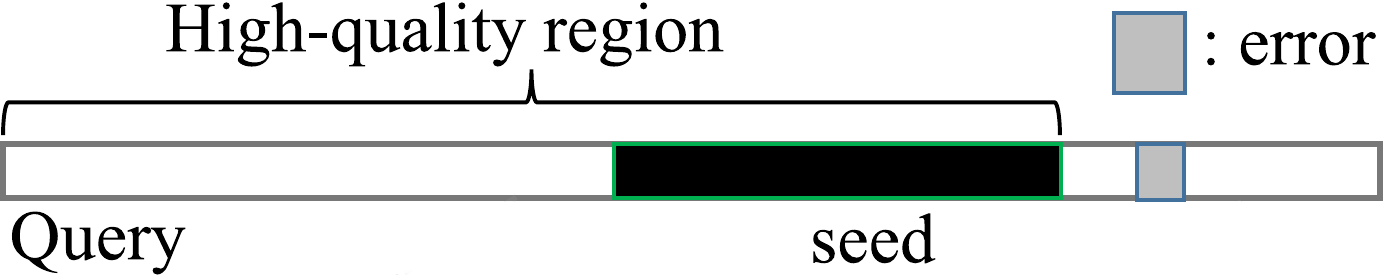
\includegraphics[]{./img/seed.png}
	\end{center}
	\caption{Visualisierung der Seed Position in einem fehlerhaften Query Read}
	\label{fig:seed}
\end{figure}

Nun werden in dem normalen FM-Index alle Reads gesucht, die den Seed enthalten. Dies wird durch eine Patternsuche erreicht und resultiert in einem zusammenhängenden Suffix-Array-Intervall aller Vorkommen des Seeds.


\subsection{Alignment der gefundenen Reads}
\label{subsec:alignment}

Zusammen mit dem vorherigen Schritt wird diese Art von Alignment als Seed-and-Extend Strategie bezeichnet.
Bereits vor dem erscheinen von FMOE wurde die FM-Index Variante dieser Strategie in der Bioinformatik verwendet.
%Quelle Fm-Index Extension
Nachdem alle Reads mit dem Seed gefunden wurden, beginnt hier also die Extension Phase.

In dieser Phase werden die gefundenen Reads Schritt für Schritt mit der Query aligned.
Man beginnt also mit dem Suffix-Array-Intervall aus dem vorherigen Schritt und führt in jedem Schritt das LF-Mapping für alle möglichen Basen (A, C, G und T) aus.
Daraus ergeben sich vier neue Intervalle, die mit dem Seed beginnen und jeweils eine weitere Base enthalten.

Auf diese Art und Weise wird ein Baum aus allen auftretenden Basen erzeugt, welche mit ihrer Intervallgröße annotiert werden (siehe Abbildung \ref{fig:extension}).
Das sorgt dafür, dass eine beliebige Menge von Reads in einen Pfad komprimiert werden, solange sie sich nicht voneinander unterscheiden.
Während dieses Prozesses werden Pfade, die zu sehr kleinen Intervallen gehören, entfernt, um das Verfahren zu beschleunigen.
Die Extension wird abgebrochen, wenn die gesamte Query enthalten ist oder die Anzahl der Pfade einen festgelegten Schwellenwert überschreitet.

Ein Beispiel für die FM-Index Extension ist in Abbildung \ref{tbl:fm-index-extension} zu sehen.

An dieser Stelle wird auch deutlich, weshalb der zweite, umgekehrte, FM-Index notwendig ist.
Die FM-Index Extension funktioniert aufgrund des LF-Mappings nur in eine Richtung. Um die Überlappung in beide Richtungen zu erweitern, ist also auch ein FM-Index der alle Reads rückwärts enthält nötig.

%TODO:Quelle original Paper
\begin{figure}[h]
	\begin{center}
		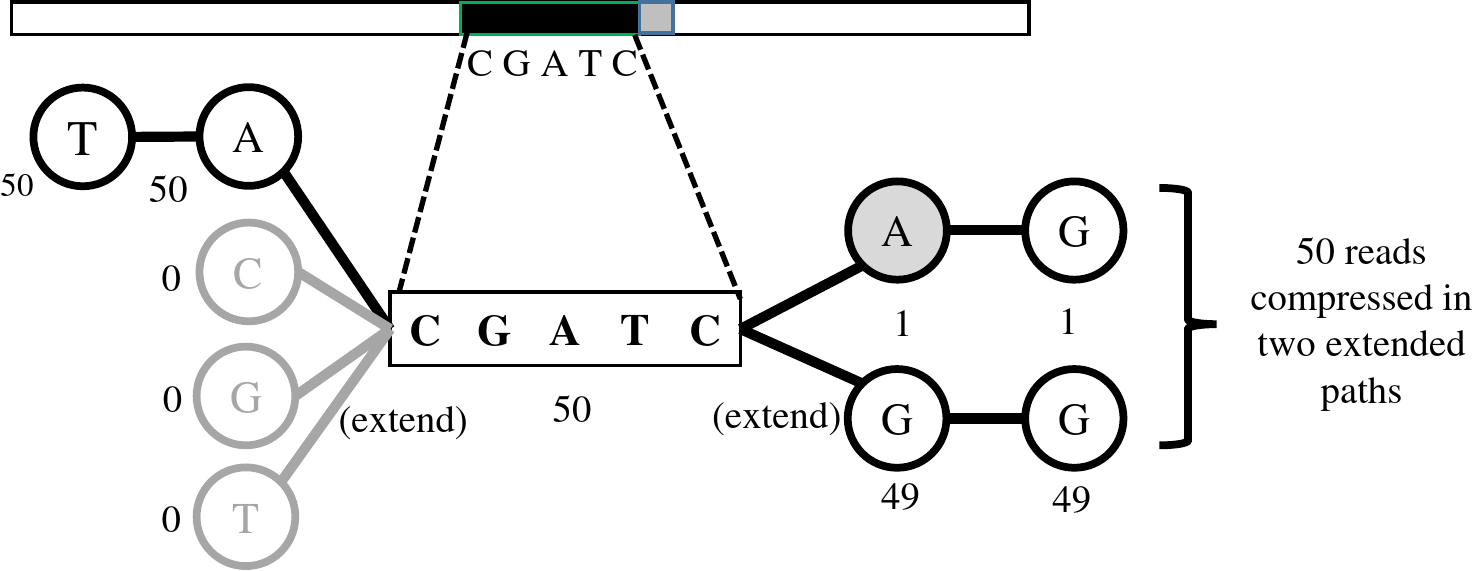
\includegraphics[]{./img/extension.png}
	\end{center}
	\caption{Extension Baum von 50 gefundenen Reads.}
	\label{fig:extension}
\end{figure}

\begin{figure}[h]
	\begin{center}
		\begin{tabular}{ a | b c c c c c c c c c c c c c b | }
			i & L &  &  &  &  &  &  &  &  &  &  &  &  &  & F \\
			\hline
			0 & \$ & a & a & t & g & \$ & a & a & t & g & \$ & c & a & t & g \\
			\hline
			1 & \$ & a & a & t & g & \$ & c & a & t & g & \$ & a & a & t & g \\
			\hline
			2 & \$ & c & a & t & g & \$ & a & a & t & g & \$ & a & a & t & g \\
			\hline
			3 & \cellcolor{RubineRed} a \tikzmark{a21} & \cellcolor{black} \color{white} a & \cellcolor{black} \color{white} t & \cellcolor{black} \color{white} g & \$ & a & a & t & g & \$ & c & a & t & g & \$ \\
			\hline
			4 & \cellcolor{RubineRed} a \tikzmark{a22} & \cellcolor{black} \color{white} a & \cellcolor{black} \color{white} t & \cellcolor{black} \color{white} g & \$ & c & a & t & g & \$ & a & a & t & g & \$ \\
			\hline
			5 & \cellcolor{black} \color{white} a & \cellcolor{black} \color{white} t & \cellcolor{black} \color{white} g & \$ & a & a & t & g & \$ & a & a & t & g & \$ & \tikzmark{c1} \cellcolor{BurntOrange} c \\
			\hline
			6 & \cellcolor{black} \color{white} a & \cellcolor{black} \color{white} t & \cellcolor{black} \color{white} g & \$ & a & a & t & g & \$ & c & a & t & g & \$ & \tikzmark{a11} \cellcolor{RubineRed} a \\
			\hline
			7 & \cellcolor{black} \color{white} a & \cellcolor{black} \color{white} t & \cellcolor{black} \color{white} g & \$ & c & a & t & g & \$ & a & a & t & g & \$ & \tikzmark{a12} \cellcolor{RubineRed} a \\
			\hline
			8 & \cellcolor{BurntOrange} c \tikzmark{c2} & \cellcolor{black} \color{white} a & \cellcolor{black} \color{white} t & \cellcolor{black} \color{white} g & \$ & a & a & t & g & \$ & a & a & t & g & \$ \\
			\hline
			9 & g & \$ & a & a & t & g & \$ & a & a & t & g & \$ & c & a & t \\
			\hline
			10 & g & \$ & a & a & t & g & \$ & c & a & t & g & \$ & a & a & t \\
			\hline
			11 & g & \$ & c & a & t & g & \$ & a & a & t & g & \$ & a & a & t \\
			\hline
			12 & t & g & \$ & a & a & t & g & \$ & a & a & t & g & \$ & c & a \\
			\hline
			13 & t & g & \$ & a & a & t & g & \$ & c & a & t & g & \$ & a & a \\
			\hline
			14 & t & g & \$ & c & a & t & g & \$ & a & a & t & g & \$ & a & a \\
			\hline
		\end{tabular}

		\begin{tikzpicture}[overlay, remember picture, yshift=.25\baselineskip, shorten >=.5pt, shorten <=.5pt]
			\draw [->, thick, blue] ({pic cs:a11}) [bend right] to ({pic cs:a21});
			\draw [->, thick, blue] ({pic cs:a12}) [bend right] to ({pic cs:a22});
			\draw [->, thick, blue] ({pic cs:c1}) [bend left] to ({pic cs:c2});
		\end{tikzpicture}

		\caption{FM-Index der Reads \glqq aatgc\grqq, \glqq aatgc\grqq und \glqq catgc\grqq mit Trennzeichen \glqq \$\grqq.
		Von dem Intervall des Seeds \glqq atgc\grqq, $[5,7]$ ausgehend, entstehen durch das LF-Mapping mit allen vorhandenen Zeichen zwei Pfade: \glqq a\grqq, $[3,4]$ und \glqq c\grqq, $[8,8]$}
		\label{tbl:fm-index-extension}
	\end{center}
\end{figure}


Anstatt das Alignment aus dem erhaltenen Baum mit herkömmlichen Verfahren aus dem Feld der dynamischen Programmierung zu berechnen, wurde eine heuristische Lösung entworfen.
Noch vor der Extension werden die Suffix-Array-Intervalle aller k-mere des Query Reads berechnet.
Während der Extension wird dann jedem neuen Pfad sein Intervall zugeordnet.

Ist das Intervall des Pfads äquivalent zu dem Intervall eines k-meres aus der Query mit gleichem Abstand vom Seed, so überlappt sich die Query mit den Reads in diesem Pfad.

An dieser Stelle müssen allerdings mögliche Indels beachtet werden, welche den effektiven Abstand des gemeinsamen k-mers vom Seed beeinflussen können.
Um eine gewisse Anzahl Indels zu tollerieren, müssen also auch Suffix-Array-Intervalle der benachbarten k-mere mit denen der Pfade verglichen werden.


\subsection{Fehlerkorrektur durch k-mer Voting}
\label{subsec:fehlerkorrektur-voting}

Üblicherweise wird nach der Berechnung eines MSA, wie im vorherigen Schritt, eine Matrix aller alignten Reads erstellt (siehe Abbildung \ref{fig:msa-voting}).
Aus dieser Matrix lässt sich die Häufigkeit jeder Base für jede alignte Position der Query berechnen.

Eine einfache Lösung, um Fehler zu beheben, wäre also, die seltenen Basen in der Query durch die Häufigsten der jeweiligen Position zu ersetzen.
Diese Vorgehensweise ist zwar weit verbreitet, sorgt unter Umständen aber für Probleme.

Die chemischen Verfahren, die aktuellen Sequenzierungsmethoden zugrunde liegen, identifizieren nicht alle Basen gleich gut.
Regionen mit hohen Guanin und Cytosin Konzentrationen lassen sich nicht so gut verstärken, wie Adenin und Thymin reiche Regionen.
Aus diesem Grund enthalten solche Regionen verstärkt Fehler.

Diese und ähnliche systematische Fehler können bei herkömmlichen MSA Matrix Verfahren dafür sorgen, dass die Häufigkeit falscher Basen, die der korrekten übersteigt.

Um dem entgegen zu wirken, verwendet FMOE an dieser Stelle sogenanntes k-mer Voting (siehe Abbildung \ref{fig:k-mer-voting}).
Beim k-mer Voting werden die k-mere aller Reads erzeugt, die die Fehlerposition enthalten. Die Häufigkeit aller unterschiedlichen k-mere wird berechnet und das Häufigste ersetzt die Fehlerposition.

Der Vorteil von k-mer Voting ist, dass selbst Reads mit hohen Fehleranteilen stückweise korrekte Sequenzen enthalten.
Diese sind statistisch häufiger als identische Fehler in mehreren Reads und sorgen so für Wahl der korrekten Base.

$k$ ist im Fall von FMOE standardmäßig 5, abhängig von der Länge des Alignments können aber andere Werte optimaler sein.
Hier müssen neben dem Rechenaufwand wieder mehrere Faktoren abgewogen werden.
Es wäre es auch möglich verschiedene Werte aus einem fetgelegten Intervall zu testen und die eindeutigste Entscheidung zu übernehmen.

Ein Algorithmisch bedingter Vorteil dieser Methode ist, dass die Häufigkeit der k-mere bereits durch die Intervallgrößen aus dem Alignmentschritt gegeben sind.
Das offensichtlich komplexere Verfahren benötigt an dieser Stelle also nicht signifikant mehr Rechenleistung.

%TODO:Quelle original Paper
\begin{figure}[h]
	\begin{center}
		\subfigure[MSA Matrix] {
				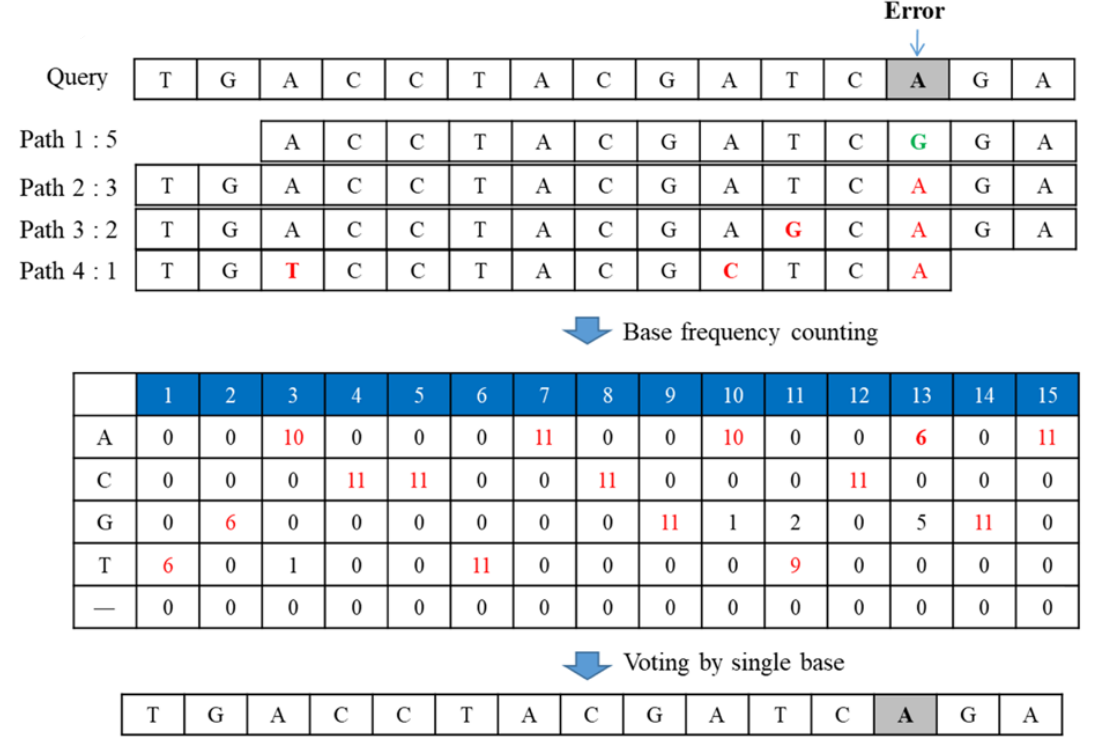
\includegraphics[width=.45\columnwidth]{./img/msa.png}
				\label{fig:msa-voting}
		}
		\subfigure[k-mer Voting] {
				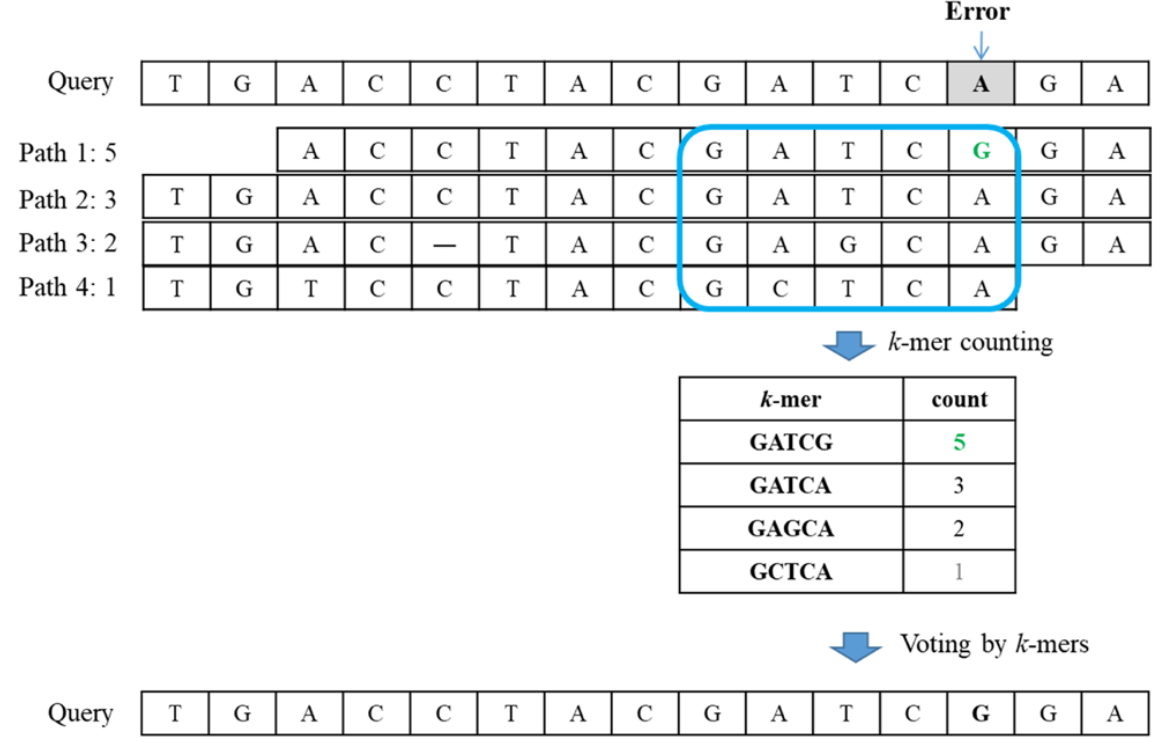
\includegraphics[width=.45\columnwidth]{./img/k-mer_voting.png}
				\label{fig:k-mer-voting}
		}
	\end{center}
	\caption{Single-Base-Voting per MSA vs. k-mer Voting}
	\label{fig:correction-voting}
\end{figure}
